\section{Spezielle Punkte und Eigenschaften von Kurven}
\subsubsection*{Einführungsaufgabe}
Betrachten Sie folgenden Graphen der Funktion $f$:
\begin{center}
    \begin{tikzpicture}
        \begin{axis}[
                width=12cm, height=12cm,
                xmin=0, xmax=7.2,
                ymin=-5, ymax=5.5,
                axis lines=middle,
                xtick={0,1,2,3,4,5,6,7},
                % ytick={-4,-3,-2,-1,0,1,2,3,4,5},
                yticklabels={},              % keine Beschriftung an der y-Achse
                xlabel={$x$}, ylabel={$y$},
                xlabel style={anchor=west},
                ylabel style={anchor=south},
                % grid=both,
                minor tick num=1,
                grid style={line width=.1pt, draw=gray!25},
                major grid style={line width=.2pt, draw=gray!45},
                clip=false,
            ]
            \addplot[thick, teal!70!black, domain=1.245:6.75, samples=300, smooth]
            {45/64*(192*x - (224/2)*x^2 + (92/3)*x^3 - 4*x^4 + (1/5)*x^5 - (1792/15))};
        \end{axis}
    \end{tikzpicture}
\end{center}
Sie wollen nun Ihrer Freundin F. über das Telefon den Graphen so beschreiben, dass F. diesen möglichst genau skizzieren kann.
\newpage
\subsection{Spezielle Punkte auf dem Graphen einer Funktion}
Vielleicht haben Sie in der Einführungsaufgabe bemerkt, dass es bestimmte Punkte auf dem Graphen von $f$ gibt, mit deren Angabe man den Graphen der Funktion qualitativ ziemlich genau zeichnen kann.
\begin{center}
    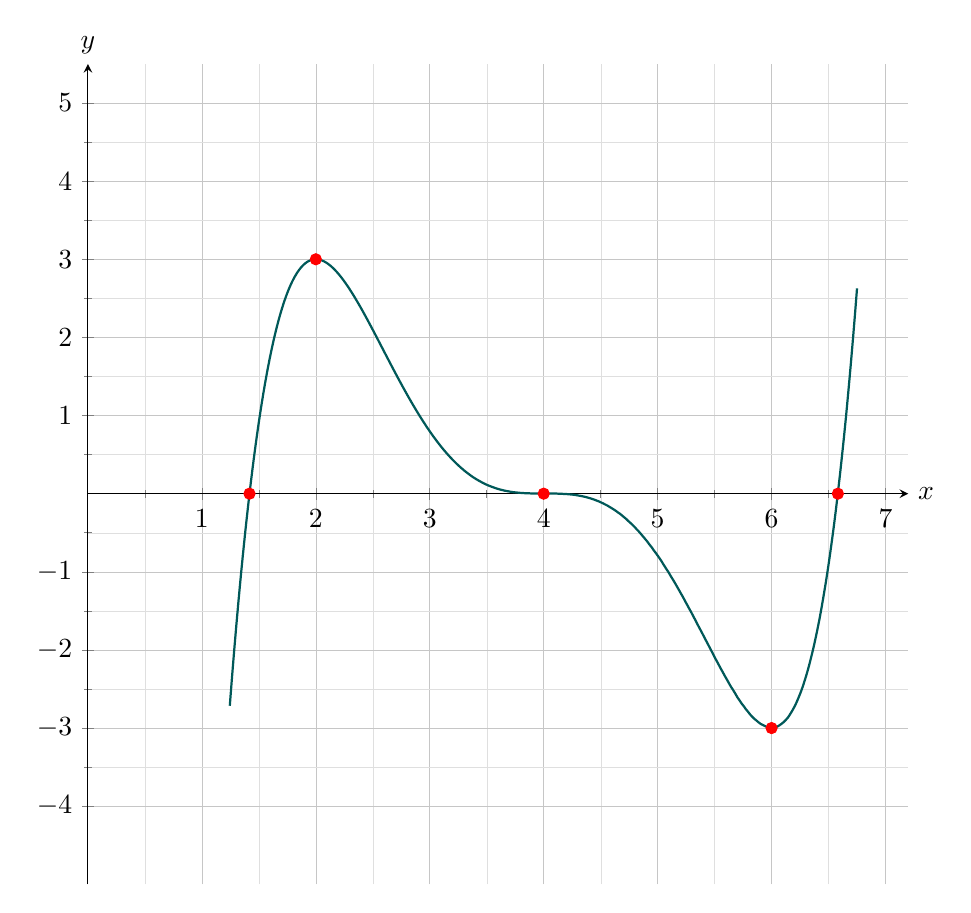
\begin{tikzpicture}
        \begin{axis}[
                width=12cm, height=12cm,
                xmin=0, xmax=7.2,
                ymin=-5, ymax=5.5,
                axis lines=middle,
                xtick={0,1,2,3,4,5,6,7},
                ytick={-4,-3,-2,-1,0,1,2,3,4,5},
                xlabel={$x$}, ylabel={$y$},
                xlabel style={anchor=west},
                ylabel style={anchor=south},
                grid=both,
                minor tick num=1,
                grid style={line width=.1pt, draw=gray!25},
                major grid style={line width=.2pt, draw=gray!45},
                clip=false,
            ]
            \addplot[thick, teal!70!black, domain=1.245:6.75, samples=300, smooth]
            {45/64*(192*x - (224/2)*x^2 + (92/3)*x^3 - 4*x^4 + (1/5)*x^5 - (1792/15))};
            \addplot[only marks, mark=*, mark size=2pt, red] coordinates {(2,3) (4,0) (6,-3) (1.418,0) (6.582,0)};
        \end{axis}
    \end{tikzpicture}
\end{center}
Natürlich reicht es nicht einfach, die Koordinaten anzugeben, sondern man muss die Punkte charakterisieren, d.h. man muss zusätzlich angeben, um was für Punkte es sich handelt. Man spricht von \textbf{Nullstelle}, \textbf{Hochpunkt}, \textbf{Tiefpunkt} und \textbf{Terrassenpunkt}.
\newpage
\begin{example}
    Skizzieren Sie mit folgenden Informationen den Graphen der Funktion:
    \begin{multicols}{3}
        \begin{description}
            \item[$P_1$:] Tiefpunkt in $(1.5,0)$
            \item[$P_2$:] Hochpunkt in $(2,3)$
            \item[$P_3$:] Nullstelle in $(4,0)$
            \item[$P_4$:] Tiefpunkt in $(6,-3)$
            \item[$P_5$:] Hochpunkt in $(6.5,0)$
        \end{description}
    \end{multicols}
    \begin{center}
        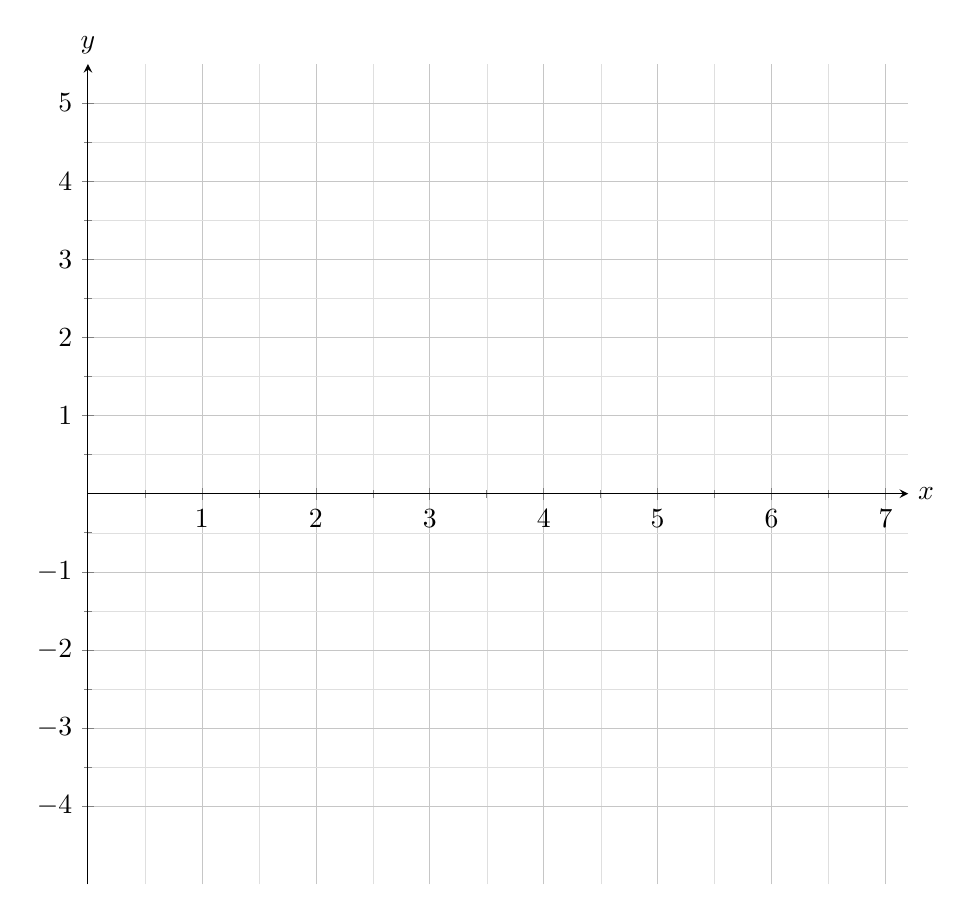
\begin{tikzpicture}
            \begin{axis}[
                    width=12cm, height=12cm,
                    xmin=0, xmax=7.2,
                    ymin=-5, ymax=5.5,
                    axis lines=middle,
                    xtick={0,1,2,3,4,5,6,7},
                    ytick={-4,-3,-2,-1,0,1,2,3,4,5},
                    xlabel={$x$}, ylabel={$y$},
                    xlabel style={anchor=west},
                    ylabel style={anchor=south},
                    grid=both,
                    minor tick num=1,
                    grid style={line width=.1pt, draw=gray!25},
                    major grid style={line width=.2pt, draw=gray!45},
                    clip=false,
                ]
            \end{axis}
        \end{tikzpicture}
    \end{center}
\end{example}
\newpage
\subsection{Die Ableitung als Diagnoseinstrument für Monotonie und Extrema}
Im letzten Abschnitt haben wir gesehen, dass die Kenntnis von den Hoch- und Tiefpunkten, Terrassenpunkte und Nullstellen einer Funktion uns in die Lage versetzen, den Graphen ziemlich akkurat zu skizzieren. In diesem Abschnitt setzen wir uns damit auseinander, wie man diese Punkt (rechnerisch) anhand der Funktionsgleichung bestimmen kann.
\subsubsection*{Einführungsaufgabe}
In den ersten sechs Koordinatensystemen (1-6) sind Ausschnitte von sechs Funktionsgraphen gezeichnet. In den sechs Koordinatensystemen darunter (A-F) Ausschnitte von sechs Ableitungen. Welche Ableitung passt zu welchem Graph?
\begin{center}
    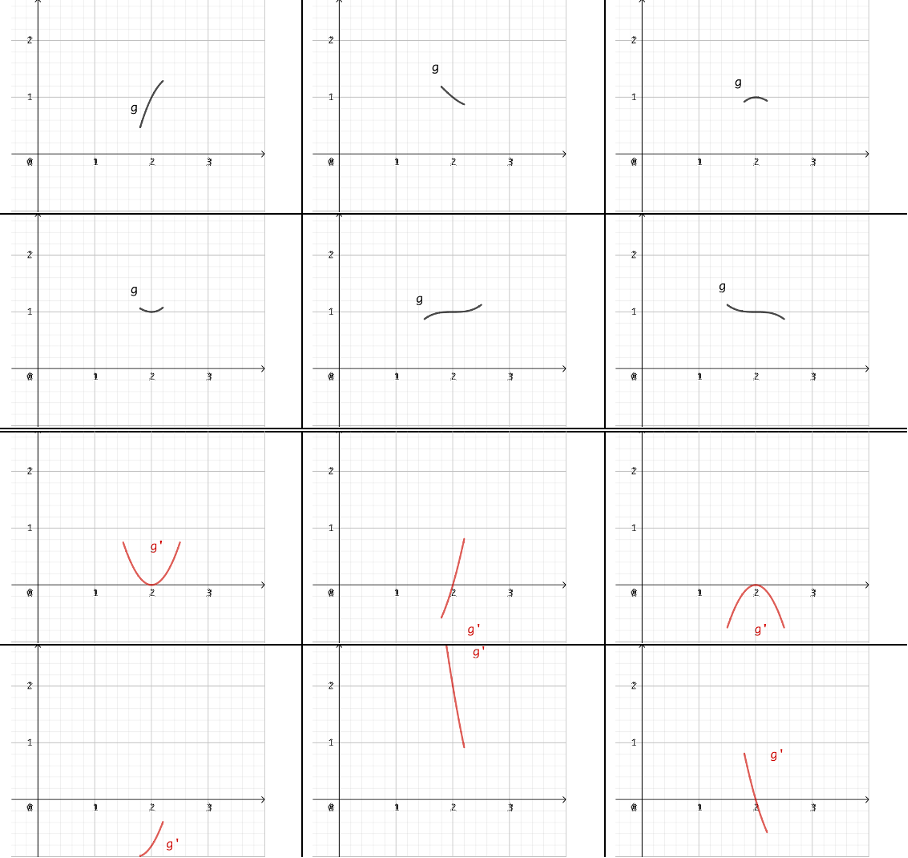
\includegraphics{im/KurvendiskussionEA.png}
\end{center}
Notieren Sie was Ihnen bei der Zuordnung geholfen hat:
\newpage
Ableitungen sind bei vielen Fragestellungen überaus nützlich. In diesem Abschnitt setzen wir sie gewissermassen als Diagnoseinstrument ein. Sie sind nämlich hervorragend geeignet, die Form von Funktionsgraphen zu diagnostizieren. Wir beginnen mit einem Beispiel.

\begin{examplebreak}
    \[f\left(x\right)=\frac{1}{3}x^3-4x^2+12x+1\] Frage: Wie sieht der Graph von f (ungefähr) aus?\\
    Da $f$ eine Funktion 3. Grades ist, können wir die Antwort nicht ohne Weiteres geben. Deswegen untersuchen wir zunächst die Ableitung:
    \begin{align*}
        \frac{df}{dx}\left(x\right)=x^2-8x+12
    \end{align*}
    \begin{minipage}{0.6\textwidth}
        Die Ableitung ist um einiges einfacher. Es handelt sich um eine quadratische Funktion. Der Graph ist eine nach oben geöffnete Parabel mit den Nullstellen
        \begin{align*}
            x_{1,2}=\frac{8\pm\sqrt{8^2-4\cdot12}}{2}=6\ \text{oder}\ 2
        \end{align*}
        Nun können wir aufgrund der Informationen über die Ableitung auf den Verlauf des Graphen von $f$ schliessen:
    \end{minipage}
    \begin{minipage}{0.4\textwidth}
        \begin{figure}[H]
            \definecolor{qqwuqq}{rgb}{0,0.39215686274509803,0}
            \begin{tikzpicture}[line cap=round,line join=round,>=triangle 45,x=1cm,y=1cm, scale=0.6]
                \begin{axis}[
                        x=1cm,y=0.5cm,
                        axis lines=middle,
                        ymajorgrids=false,
                        xmajorgrids=false,
                        xmin=-0.5,
                        xmax=8.2,
                        ymin=-4.5,
                        ymax=10.5,
                        xtick={0,1,...,8},
                        ytick={-4,-2,...,10},]
                    \clip(-0.5,-4.5) rectangle (8.2,10.5);
                    \draw[line width=2pt,color=qqwuqq,smooth,samples=100,domain=-0.5:8.2] plot(\x,{(\x)^(2)-8*(\x)+12});
                    \begin{scriptsize}
                        \draw[color=qqwuqq] (0.6,10.0) node {$f'$};
                    \end{scriptsize}
                \end{axis}
            \end{tikzpicture}
        \end{figure}
        \vspace{0.3cm}
    \end{minipage}
    \textbf{Für $\boldsymbol{x<2}$ ist $\boldsymbol{f^\prime\left(x\right)>0}$.}\\
    In diesem Bereich hat der Graph von f also immer eine positive Steigung. Oder anders gesagt: $f$ ist im Bereich $]-\infty,2[$  monoton wachsend.\\
    \vspace{0.5cm}

    \textbf{An der Stelle $\boldsymbol{x=2}$ wechselt die Ableitung von positiv nach negativ.}\\
    Die Funktion $f$ ist also davor steigend und nachher fallend. An dieser Stelle hat den Graph von $f$ einen Hochpunkt!
    \begin{align*}
        H=(2, f(2))=(2, 11.\bar{6})
    \end{align*}\\
    \vspace{0.5cm}

    \textbf{Für $\boldsymbol{2 < x < 6}$ ist die Ableitung negativ.}\\
    Die Funktion $f$ ist in diesem Bereich monoton fallend.\\
    \vspace{0.5cm}

    \textbf{Bei $\boldsymbol{x=6}$ wechselt das Vorzeichen der Ableitung erneut, diesmal von negativ nach positiv.} Der Graph von $f$ ist kurz vor $4$ noch fallend, nachher steigend. An dieser Stelle hat $f$ einen Tiefpunkt
    \[
        T = (6, f(6))=(6, 1)
    \]
    \vspace{0.5cm}

    \textbf{Für $\boldsymbol{x>6}$ sind die Werte der Ableitung positiv.}\\
    Die Funktion $f$ ist in diesem Bereich wieder monoton wachsend.\\
    \vspace{0.5cm}

    Mit diesen Informationen erhält man schon einen guten Eindruck über die Gestalt des Graphen von $f$.
    \begin{figure}[H]
        \definecolor{qqwuqq}{rgb}{0,0.39215686274509803,0}
        \begin{tikzpicture}[line cap=round,line join=round,>=triangle 45,x=1cm,y=1cm]
            \begin{axis}[
                    x=1cm,y=0.5cm,
                    axis lines=middle,
                    ymajorgrids=false,
                    xmajorgrids=false,
                    xmin=-0.5,
                    xmax=8.610429447852761,
                    ymin=-0.4999999999999997,
                    ymax=11.899999999999999,
                    xtick={0,1,...,8},
                    ytick={0,5,10},]
                \clip(-0.5,-0.5) rectangle (8.610429447852761,11.9);
                \draw[line width=2pt,color=qqwuqq,smooth,samples=100,domain=-0.5:8.610429447852761] plot(\x,{1/3*(\x)^(3)-4*(\x)^(2)+12*(\x)+1});
                \begin{scriptsize}
                    \draw[color=qqwuqq] (0.2,1) node {$f$};
                    \draw [fill=blue] (2,11.666666666666666) circle (2.5pt);
                    \draw[color=blue] (2,11) node {$H$};
                    \draw [fill=red] (6,1) circle (2.5pt);
                    \draw[color=red] (6,1.6) node {$T$};
                \end{scriptsize}
            \end{axis}
        \end{tikzpicture}
    \end{figure}
\end{examplebreak}

\definecolor{ccqqqq}{rgb}{0.8,0,0}
\begin{table}[H]
    \centering
    \begin{tabular}{|c|c|}
        \hline
        \textbf{Zusammenfassung der ersten Erkenntnisse}                                   & \textbf{Graph von} $\boldsymbol{F}$                                                                         \\
        \hline
        \begin{minipage}{0.7\textwidth}
            \vspace{0.2cm}
            Sei $f$ eine differenzierbare Funktion mit Definitionsbereich $\mathbb{D}_f$.\\ Sei $I$ ein Intervall $I\subset\mathbb{D}_f$ und $x_0\in D_f$.
        \end{minipage}
                                                                                           &                                                                                                             \\
        \hline
        \begin{minipage}{0.7\textwidth}
            f ist im Intervall $I$ \textbf{streng monoton wachsend}\\
            $\Leftrightarrow$\\
            $f^\prime\left(x\right)>0$ für alle $x\in I$
        \end{minipage}                          & \raisebox{-0.5\totalheight}{\begin{tikzpicture}[line cap=round,line join=round,>=triangle 45,x=1cm,y=1cm]
                                                                                      \clip(1,1.1) rectangle (3,3.9);
                                                                                      \draw[line width=2pt,color=ccqqqq,smooth,samples=100,domain=1:3] plot(\x,{2*sqrt((\x))});
                                                                                  \end{tikzpicture}}                                   \\
        \hline
        \begin{minipage}{0.7\textwidth}
            \vspace{0.5cm}
            f ist im Intervall $I$ \textbf{streng monoton fallend}\\
            $\Leftrightarrow$\\
            $f^\prime\left(x\right) < 0$ für alle $x\in I$
            \vspace{0.5cm}
        \end{minipage}                           & \raisebox{-0.5\totalheight}{\begin{tikzpicture}[line cap=round,line join=round,>=triangle 45,x=3cm,y=3cm]
                                                                                       \clip(0.8231714750413085,0.2473708885028528) rectangle (1.3714820822358982,0.7297643735210458);
                                                                                       \draw[line width=2pt,color=ccqqqq,smooth,samples=100,domain=0.8231714750413085:1.3714820822358982] plot(\x,{0.5*1/(\x)});
                                                                                   \end{tikzpicture}}  \\
        \hline
        \begin{minipage}{0.7\textwidth}
            f hat an der Stelle $x_0$ ein \textbf{lokales Maximum} (oder \textbf{Hochpunkt})\\
            $\Leftrightarrow$\\
            $f'$ wechselt an der Stelle $x_0$ das Vorzeichen von positiv zu negativ.
            \vspace{0.5cm}
        \end{minipage} & \raisebox{-0.2\totalheight}{\begin{tikzpicture}[line cap=round,line join=round,>=triangle 45,x=1cm,y=1cm]
                                                             \clip(-1.1776622854217196,-1.422473266062714) rectangle (1.189011787128655,0.6596826119734079);
                                                             \draw [samples=50,rotate around={-180:(0,0)},xshift=0cm,yshift=0cm,line width=2pt,domain=-1.5:1.5), color=ccqqqq] plot (\x,{(\x)^2/2/0.25});
                                                         \end{tikzpicture}}    \\
        \hline
        \begin{minipage}{0.7\textwidth}
            \vspace{0.5cm}
            f hat an der Stelle $x_0$ ein \textbf{lokales Minimum} (oder \textbf{Tiefpunkt})\\
            $\Leftrightarrow$\\
            $f'$ wechselt an der Stelle $x_0$ das Vorzeichen von negativ zu positiv.
            \vspace{0.5cm}
        \end{minipage} & \raisebox{-0.6\totalheight}{\begin{tikzpicture}[line cap=round,line join=round,>=triangle 45,x=1cm,y=1cm]
                                                             \clip(-1.1776622854217196,-1.422473266062714) rectangle (1.189011787128655,0.6596826119734079);
                                                             \draw [samples=50,rotate around={-180:(0,0)},xshift=0cm,yshift=0.7cm,line width=2pt,domain=-1.5:1.5), color=ccqqqq] plot (\x,{-(\x)^2/2/0.25});
                                                         \end{tikzpicture}} \\
        \hline
    \end{tabular}
\end{table}
\newpage
\subsubsection{Übungen}
\begin{enumerate}
    \item Machen Sie eine Skizze des Graphen von f, indem Sie die Ableitung untersuchen:
          \begin{enumerate}
              \item $f\left(x\right)=2x^3-3x^2-36x$
              \item $g\left(x\right)=\frac{1}{3}x^3-4x^2+16x$
              \item $h\left(x\right)=-x^3$
          \end{enumerate}
    \item In der 2. Klasse haben Sie gelernt, dass der Scheitelpunkt einer Parabel der Form
          \[f:\ \ y=ax^2+bx+c\] an der Stelle $x_s=-\frac{b}{2a}$ liegt.\\
          Beweisen Sie diesen Sachverhalt unter Verwendung der Ableitung.
    \item An welcher Stelle fällt der Graph von $f\left(x\right)=2x^3-3x^2-36x$ am steilsten?
\end{enumerate}
\clearpage
\subsection{Spezielle Punkte bestimmen}
Um zu bestimmen, ob eine Funktion $f$ an einer Stelle $x_0$ ein lokales Maximum oder Minimum hat, muss analysiert werden, ob $f'$ an der Stelle $x_0$ das Vorzeichen von $+$ zu $-$ wechselt oder umgekehrt (siehe letzter Abschnitt). Dies kann in der Praxis kompliziert sein. Häufiger ist es einfacher, wenn man dazu die Ableitungsfunktion nochmals ableitet.

Wie kann man nun mit den höheren Ableitungen entscheiden, ob $f'$ an einer bestimmten Stelle das Vorzeichen von $+$ nach $-$ oder umgekehrt wechselt? Betrachten Sie dazu das folgende Beispiel:

\begin{example}
    Wie sieht der Graph einer Funktion $f$ in der Umgebung von $x = 1$ aus, wenn $f(1) = 4$, $f'(1) =0$ und $f''(1) = 2$ ist?
    \begin{center}
        \begin{tikzpicture}[scale=1.3, every node/.style={font=\small}]

            % --- Koordinatensystem 1: f'' ---
            \begin{scope}[xshift=0cm]
                \draw[-{Latex}] (-0.5,0) -- (2.5,0) node[right] {$x$};
                \draw[-{Latex}] (0,-0.8) -- (0,2.3) node[above] {$y$};
                \node[above] at (1.5,1.3) {$f''$};
                \draw (0,1) -- (-0.05,1) node[left] {$2$};
                \draw (1.5,0) -- (1.5,-0.05) node[below] {$1$};
                \filldraw[black] (1.5,1) circle (1.5pt);
            \end{scope}

            % Pfeil 1
            \draw[-{Latex}, thick] (2.7,1) -- (3.4,1);

            % --- Koordinatensystem 2: f' ---
            \begin{scope}[xshift=4cm]
                \draw[-{Latex}] (-0.5,0) -- (2.5,0) node[right] {$x$};
                \draw[-{Latex}] (0,-0.8) -- (0,2.3) node[above] {$y$};
                \node[above] at (1.5,1.3) {$f'$};
                % \draw (0,1) -- (-0.05,1) node[left] {$2$};
                \draw (1.5,0) -- (1.5,-0.05) node[below] {$1$};
                \filldraw[black] (1.5,0) circle (1.5pt);
            \end{scope}

            % Pfeil 2
            \draw[-{Latex}, thick] (6.7,1) -- (7.4,1);

            % --- Koordinatensystem 3: f ---
            \begin{scope}[xshift=8cm]
                \draw[-{Latex}] (-0.5,0) -- (2.5,0) node[right] {$x$};
                \draw[-{Latex}] (0,-0.8) -- (0,2.3) node[above] {$y$};
                \node[above] at (1.5,1.3) {$f$};
                % \draw (0,1) -- (-0.05,1) node[left] {$2$};
                \draw (0,2) -- (-0.05,2) node[left] {$4$};
                \draw (1.5,0) -- (1.5,-0.05) node[below] {$1$};
                \filldraw[black] (1.5,2) circle (1.5pt);
            \end{scope}

        \end{tikzpicture}
    \end{center}
\end{example}
\subsubsection*{Krümmung}
Stellen Sie sich den Graphen als eine Strasse vor. Wir fahren nun mit einem Auto von links nach rechts entlang des Graphen.
\begin{center}
    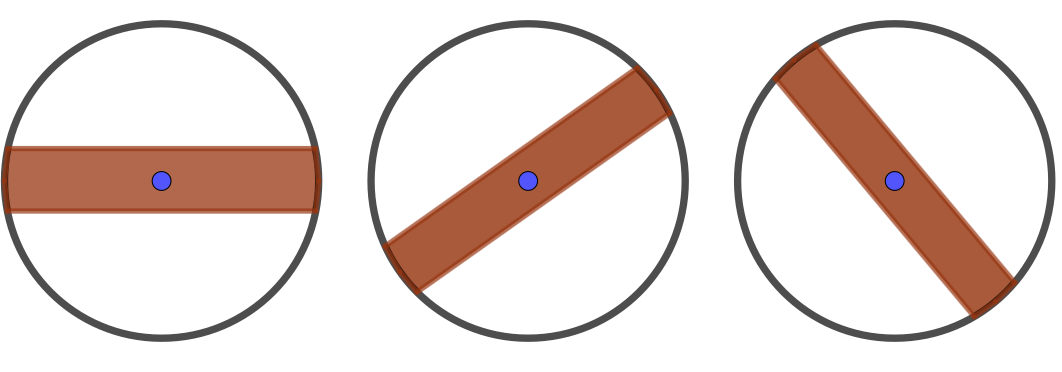
\includegraphics[width=0.5\textwidth]{im/KruemmungLenkrad.png}
\end{center}
Wenn wir geradeaus fahren, dann sieht das Steuerrad aus wie in der obigen Abbildung links. Wenn wir aber eine Linkskurve fahren, dann ist das Steuerrad verdreht wie in der mittleren Abbildung. Dann nennen wir die Kurve \textbf{linksgekrümmt}. Wenn wir uns in einer Rechtskurve befinden, dann ist das Steuerrad verdreht wie in der Abbildung rechts. In diesem Fall nennen wir die Kurve \textbf{rechtsgekrümmt}.

Wenn wir nun eine Funktion betrachten, deren Graph in einem bestimmten Intervall linksgekrümmt ist, dann nehmen - von links nach rechts betrachtet - die Funktionswerte der ersten Ableitung immer nur zu: Legen Sie dazu in Gedanken eine Tangente an den linksgekrümmten Graphen und verfolgen Sie, wie deren Steigung sich verändert. Eine Linkskrümmung lässt sich also dadurch charakterisieren, dass die erste Ableitung streng monoton wächst. Analog dazu lässt sich eine Rechtskrümmung dadurch charakterisieren, dass die erste Ableitung streng monoton sinkt.

\subsubsection*{Wendepunkt} Punkt auf dem Graphen mit der Eigenschaft, dass der Graph vorher links- und nachher rechtsgekrümmt ist, oder umgekehrt. Das Krümmungsverhalten wechselt also in einem solchen Punkt.
\subsubsection*{Mathematische Definitionen}
\begin{deff}[Krümmung]{}
    \begin{center}
        \begin{table}[H]
            \centering
            \begin{tabular}{|c|c|}
                \hline
                \begin{minipage}{0.7\textwidth}
                    \vspace{0.2cm}
                    $f$ ist im Intervall $I$ \textbf{linksgekrümmt} (oder \textbf{konvex})\\
                    $\Leftrightarrow$\\
                    $f''(x) > 0$ für alle $x \in I$
                    \vspace{0.2cm}
                \end{minipage}
                 & \raisebox{-0.5\totalheight}{\begin{tikzpicture}[scale=0.7,line cap=round,line join=round,>=triangle 45,x=1cm,y=1cm]
                                                       \draw[-{Stealth[length=2mm]}, gray] (-0.4,0) -- (4.2,0);
                                                       \draw[-{Stealth[length=2mm]}, gray] (0,-0.3) -- (0,4.3);
                                                       \draw[line width=1.5pt, color=ccqqqq, smooth, samples=60, domain=0.7:4]
                                                       plot(\x,{6/(\x+0.55)-0.3});
                                                       \draw[blue, ultra thick] (1.6,0) -- (3.4,0);
                                                       \node[blue, below] at (2.5,-0.05) {\scriptsize $I$};
                                                   \end{tikzpicture}} \\
                \hline
                \begin{minipage}{0.7\textwidth}
                    \vspace{0.2cm}
                    $f$ ist im Intervall $I$ \textbf{rechtsgekrümmt} (oder \textbf{konkav})\\
                    $\Leftrightarrow$\\
                    $f''(x) < 0$ für alle $x \in I$
                    \vspace{0.2cm}
                \end{minipage}
                 & \raisebox{-0.5\totalheight}{\begin{tikzpicture}[scale=0.7,line cap=round,line join=round,>=triangle 45,x=1cm,y=1cm]
                                                       \draw[-{Stealth[length=2mm]}, gray] (-0.6,0) -- (4.2,0);
                                                       \draw[-{Stealth[length=2mm]}, gray] (0,-0.6) -- (0,4.3);
                                                       \draw[line width=1.5pt, color=ccqqqq, smooth, samples=60, domain=-0.5:4]
                                                       plot(\x,{-0.55*(\x-1.3)^2+3.6});
                                                       \draw[blue, ultra thick] (1.6,0) -- (3.3,0);
                                                       \node[blue, below] at (2.45,-0.05) {\scriptsize $I$};
                                                   \end{tikzpicture}} \\
                \hline
                \begin{minipage}{0.7\textwidth}
                    \vspace{0.2cm}
                    $f$ hat an der Stelle $x_0$ einen \textbf{Wendepunkt}\\
                    $\Leftrightarrow$\\
                    $f''$ wechselt an der Stelle $x_0$ das Vorzeichen.
                    \vspace{0.2cm}
                \end{minipage}
                 & \raisebox{-0.5\totalheight}{\begin{tikzpicture}[scale=0.7,line cap=round,line join=round,>=triangle 45,x=1cm,y=1cm]
                                                       \draw[-{Stealth[length=2mm]}, gray] (-0.8,0) -- (4.8,0);
                                                       \draw[-{Stealth[length=2mm]}, gray] (0,-1.5) -- (0,3.6);
                                                       \draw[color=ccqqqq, line width=1.5pt, samples=80, domain=-0.6:4.6]
                                                       plot(\x,{0.2*(\x-2)^3 - 1.3*(\x-2) + 0.9});
                                                       \filldraw[white, draw=ccqqqq] (2,0.9) circle (2pt);
                                                       \node[color=ccqqqq, above right] at (2.05,1.05) {\scriptsize W};
                                                       \draw (2,0.05) -- (2,-0.05);
                                                       \node[below] at (2,-0.15) {\scriptsize $x_0$};
                                                   \end{tikzpicture}} \\
                \hline
            \end{tabular}
        \end{table}
    \end{center}
\end{deff}
\newpage
% Obwohl es unendlich viele Graphen gibt, können die einzelnen Abschnitte fast aller Graphen mithilfe der folgenden Beschreibungen charakterisiert werden:
% \begin{center}
%     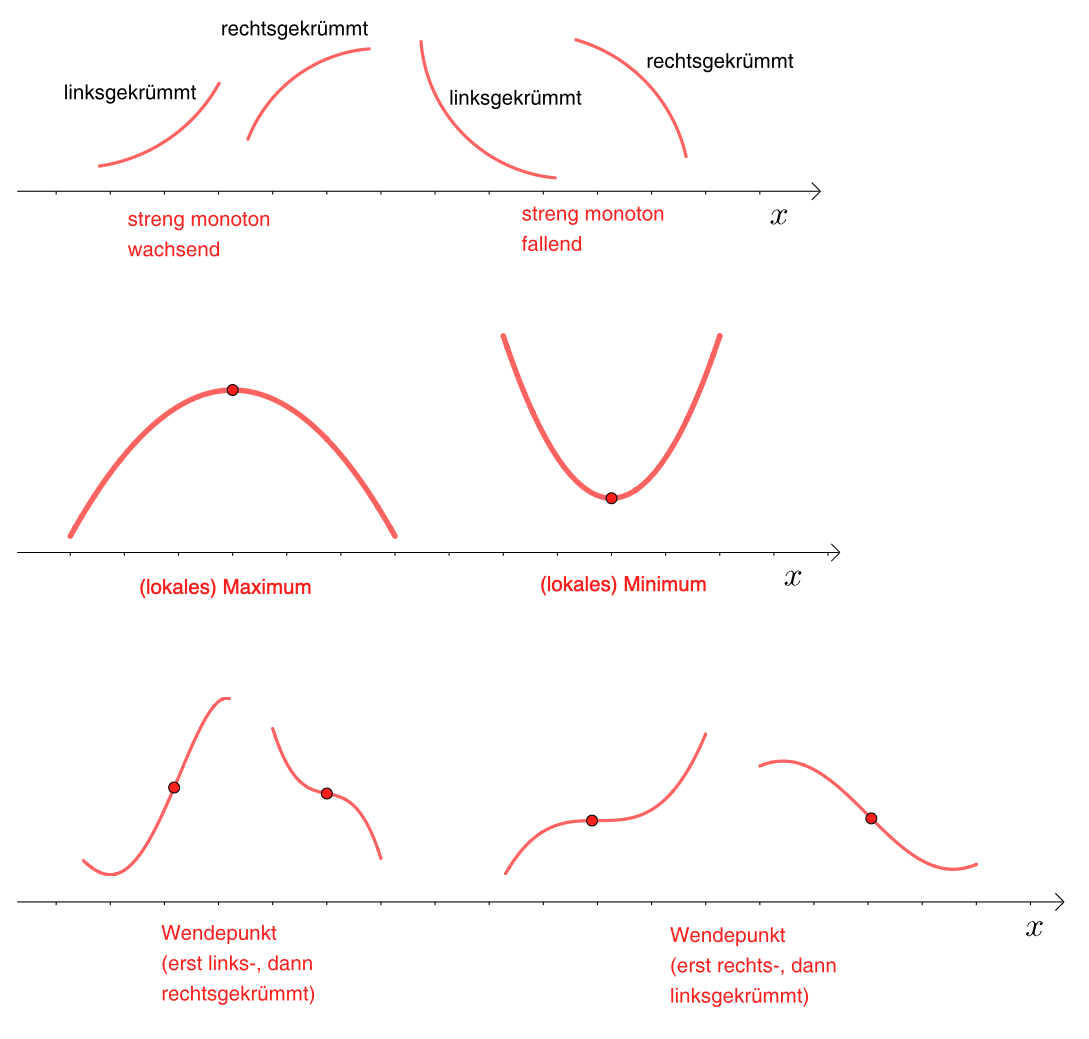
\includegraphics[width=0.8\textwidth]{im/KruemmungMaxMin.png}
% \end{center}
% \subsubsection*{Krümmung}
% Stellen Sie sich den Graphen als eine Strasse vor. Wir fahren nun mit einem Auto von links nach rechts entlang des Graphen.
% \begin{center}
%     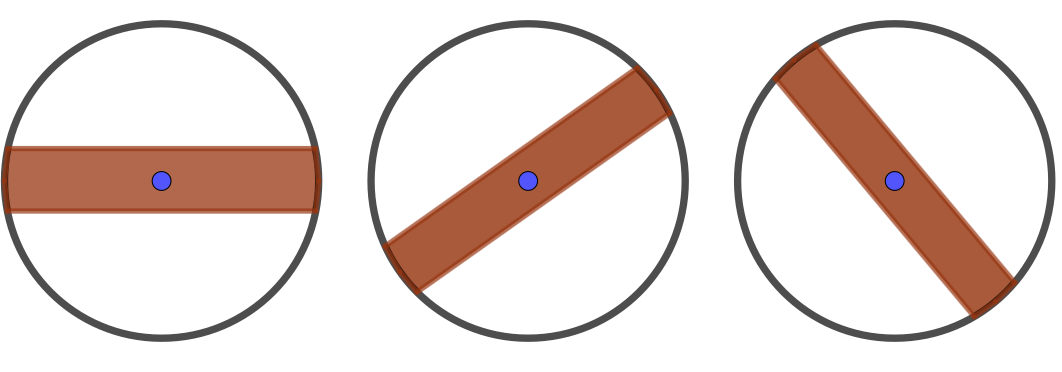
\includegraphics[width=0.5\textwidth]{im/KruemmungLenkrad.png}
% \end{center}
% Wenn wir geradeaus fahren, dann sieht das Steuerrad aus wie in der obigen Abbildung links. Wenn wir aber eine Linkskurve fahren, dann ist das Steuerrad verdreht wie in der mittleren Abbildung. Dann nennen wir die Kurve \textbf{linksgekrümmt}. Wenn wir uns in einer Rechtskurve befinden, dann ist das Steuerrad verdreht wie in der Abbildung rechts. In diesem Fall nennen wir die Kurve \textbf{rechtsgekrümmt}.

% Wenn wir nun eine Funktion betrachten, deren Graph in einem bestimmten Intervall linksgekrümmt ist, dann nehmen - von links nach rechts betrachtet - die Funktionswerte der ersten Ableitung immer nur zu: Legen Sie dazu in Gedanken eine Tangente an den linksgekrümmten Graphen und verfolgen Sie, wie deren Steigung sich verändert. Eine Linkskrümmung lässt sich also dadurch charakterisieren, dass die erste Ableitung streng monoton wächst. Analog dazu lässt sich eine Rechtskrümmung dadurch charakterisieren, dass die erste Ableitung streng monoton sinkt.

% \subsubsection*{Wendepunkt} Punkt auf dem Graphen mit der Eigenschaft, dass der Graph vorher links- und nachher rechtsgekrümmt ist, oder umgekehrt. Das Krümmungsverhalten wechselt also in einem solchen Punkt.

% \subsubsection*{lokales Maximum/Minimum (lokales Extremum)} 
% Eine Funktion hat einer bestimmten Stelle ein (lokales) Maximum, wenn an dieser Stelle (wenigstens lokal) der grösste Funktionswert vorkommt, dass also in einer bestimmten Umgebung um diese Stelle alle Funktionswerte kleiner sind. Analoges lässt sich über ein (lokales) Minimum sagen.
\subsubsection{Kriterien für spezielle Punkte finden}
Versuchen Sie selbst, die Informationen von links nach rechts zu übertragen, und skizzieren
Sie den Graphen in einer Umgebung der markierten Punkte (mit Ausnahme der Graphen
ganz links)

% Zeile a)
\begin{tikzpicture}[line cap=round, line join=round, >=Stealth, x=1cm, y=1cm, scale=1.2]
    \node at (-1.3,1) {\large a)};

    \begin{scope}[xshift=0cm]
        \draw[-{Stealth[length=2mm]}] (-0.4,0) -- (2.7,0);
        \draw[-{Stealth[length=2mm]}] (0,-1.1) -- (0,1.8);
        \node at (1.6,1.6) {$f''$};
        \draw (1.3,0.05) -- (1.3,-0.05);
        \node[above] at (1.3,0) {\scriptsize $2$};
        \fill (1.3,-0.55) circle (1.4pt);
    \end{scope}

    \begin{scope}[xshift=3.9cm]
        \draw[-{Stealth[length=2mm]}] (-0.4,0) -- (2.7,0);
        \draw[-{Stealth[length=2mm]}] (0,-1.1) -- (0,1.8);
        \node at (1.6,1.6) {$f'$};
        \fill (1.3,0) circle (1.4pt);
        \node[below] at (1.3,-0.2) {\scriptsize $2$};
    \end{scope}

    \begin{scope}[xshift=7.8cm]
        \draw[-{Stealth[length=2mm]}] (-0.4,0) -- (2.7,0);
        \draw[-{Stealth[length=2mm]}] (0,-1.1) -- (0,1.8);
        \node at (1.6,1.6) {$f$};
        \fill (1.3,0.5) circle (1.4pt);
        \draw (1.3,0.05) -- (1.3,-0.05);
        \node[below] at (1.3,-0.2) {\scriptsize $2$};
    \end{scope}
\end{tikzpicture}

\vspace{2em}

% Zeile b)
\begin{tikzpicture}[line cap=round, line join=round, >=Stealth, x=1cm, y=1cm, scale=1.1]
    \node at (-1.3,1) {\large b)};

    \begin{scope}[xshift=0cm]
        \draw[-{Stealth[length=2mm]}] (-0.4,0) -- (2.7,0);
        \draw[-{Stealth[length=2mm]}] (0,-1.1) -- (0,1.8);
        \node at (1.6,1.6) {$f'''$};
        \draw (1.3,0.05) -- (1.3,-0.05);
        \node[above] at (1.3,0) {\scriptsize $2$};
        \fill (1.3,-0.55) circle (1.4pt);
    \end{scope}

    \begin{scope}[xshift=3.4cm]
        \draw[-{Stealth[length=2mm]}] (-0.4,0) -- (2.7,0);
        \draw[-{Stealth[length=2mm]}] (0,-1.1) -- (0,1.8);
        \node at (1.6,1.6) {$f''$};
        \fill (1.3,0) circle (1.4pt);
        \node[below] at (1.3,-0.2) {\scriptsize $2$};
    \end{scope}

    \begin{scope}[xshift=6.8cm]
        \draw[-{Stealth[length=2mm]}] (-0.4,0) -- (2.7,0);
        \draw[-{Stealth[length=2mm]}] (0,-1.1) -- (0,1.8);
        \node at (1.6,1.6) {$f'$};
        \fill (1.3,0.5) circle (1.4pt);
        \draw (1.3,0.05) -- (1.3,-0.05);
        \node[below] at (1.3,-0.2) {\scriptsize $2$};
    \end{scope}

    \begin{scope}[xshift=10.2cm]
        \draw[-{Stealth[length=2mm]}] (-0.4,0) -- (2.7,0);
        \draw[-{Stealth[length=2mm]}] (0,-1.1) -- (0,1.8);
        \node at (1.6,1.6) {$f$};
        \fill (1.3,1.2) circle (1.4pt);
        \draw (1.3,0.05) -- (1.3,-0.05);
        \node[below] at (1.3,-0.2) {\scriptsize $2$};
    \end{scope}
\end{tikzpicture}

\vspace{2em}

% Zeile c)
\begin{tikzpicture}[line cap=round, line join=round, >=Stealth, x=1cm, y=1cm, scale=1.1]
    \node at (-1.3,1) {\large c)};

    \begin{scope}[xshift=0cm]
        \draw[-{Stealth[length=2mm]}] (-0.4,0) -- (2.7,0);
        \draw[-{Stealth[length=2mm]}] (0,-1.1) -- (0,1.8);
        \node at (1.6,1.6) {$f'''$};
        \fill (1.3,1.2) circle (1.4pt);
        \draw (1.3,0.05) -- (1.3,-0.05);
        \node[below] at (1.3,-0.2) {\scriptsize $2$};
    \end{scope}

    \begin{scope}[xshift=3.4cm]
        \draw[-{Stealth[length=2mm]}] (-0.4,0) -- (2.7,0);
        \draw[-{Stealth[length=2mm]}] (0,-1.1) -- (0,1.8);
        \node at (1.6,1.6) {$f''$};
        \fill (1.3,0) circle (1.4pt);
        \node[below] at (1.3,-0.2) {\scriptsize $2$};
    \end{scope}

    \begin{scope}[xshift=6.8cm]
        \draw[-{Stealth[length=2mm]}] (-0.4,0) -- (2.7,0);
        \draw[-{Stealth[length=2mm]}] (0,-1.1) -- (0,1.8);
        \node at (1.6,1.6) {$f'$};
        \fill (1.3,0) circle (1.4pt);
        \node[below] at (1.3,-0.2) {\scriptsize $2$};
    \end{scope}

    \begin{scope}[xshift=10.2cm]
        \draw[-{Stealth[length=2mm]}] (-0.4,0) -- (2.7,0);
        \draw[-{Stealth[length=2mm]}] (0,-1.1) -- (0,1.8);
        \node at (1.6,1.6) {$f$};
        \fill (1.3,0.5) circle (1.4pt);
        \draw (1.3,0.05) -- (1.3,-0.05);
        \node[below] at (1.3,-0.2) {\scriptsize $2$};
    \end{scope}
\end{tikzpicture}

% \paragraph{Krümmung}

% Wir haben im letzten Abschnitt bereits bemerkt, dass eine Funktion $f$ im Intervall $I$
% \begin{itemize}
%     \item streng monoton wachsend ist, genau dann wenn $f'(x) > 0$ für alle $x \in I$
%     \item streng monoton fallend ist, genau dann wenn $f'(x) < 0$ für alle $x \in I$
% \end{itemize}
% Dies hilft uns nun beim Diagnostizieren der Krümmung:
% \begin{center}
%     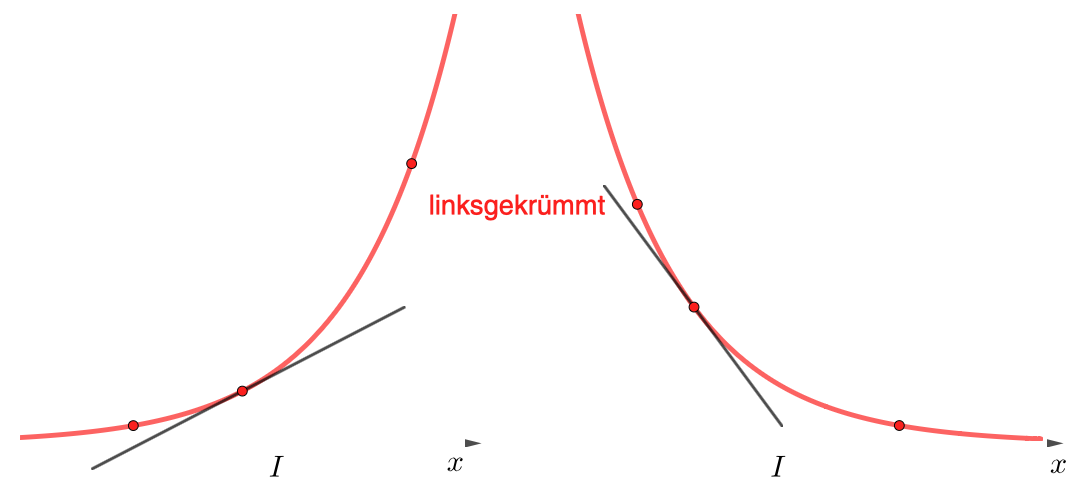
\includegraphics[width=0.8\textwidth]{im/KruemmungLinks.png}
% \end{center}
% \begin{itemize}
%     \item Linkskrümmung bedeutet ja, dass die erste Ableitung streng monoton wächst. Von links nach rechts gesehen nimmt die Steigung der Tangente immer nur zu. Damit das passiert, muss, wie wir eben gesehen haben, die Ableitung der Ableitung, also die zweite Ableitung der Ausgangsfunktion, im ganzen Intervall positiv sein: $f''(x)>0$ für alle $x\in I$.
%     \item Für die Rechtskrümmung gilt analog: $f''(x)<0$ für alle $x\in I$.
% \end{itemize}
% \subsubsection*{Extrema}

% Eine notwendige Bedingung dafür, dass an der Stelle $x_0$ ein Minimum vorliegt, ist natürlich $f'(x_0)=0$. Die Tangente an den Graphen im Punkt $(x_0,f(x_0))$ muss ja horizontal sein, also Steigung $0$ aufweisen. $x_0$ ist somit eine Nullstelle der 1. Ableitung.
% \begin{center}
%     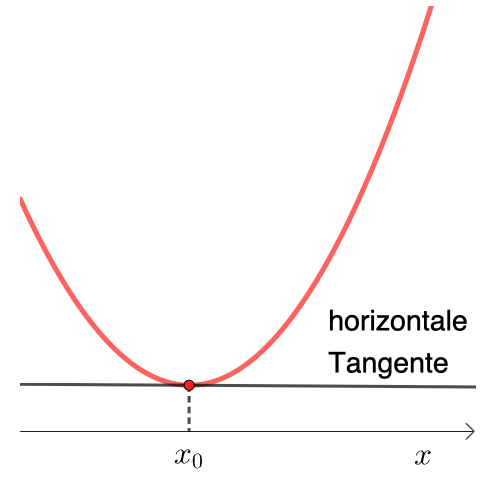
\includegraphics[width=0.3\textwidth]{im/MinimumTangenteNull.png}
% \end{center}
% \begin{minipage}{0.6\textwidth}
%     Weiter: Das hier gewünschte Kurvenverhalten (negative Steigung für $x<x_0$, Steigung $0$ an der Stelle $x_0$ und positive Steigung für $x>x_0$) können wir sicher dadurch erzwingen, dass wir $f''(x_0)>0$ verlangen, denn ist der Graph von $f'$ um $x_0$ herum monoton steigend, folglich kreuzt der Graph von $f'$ dann die $x$-Achse an der Stelle $x_0$ von links unten nach rechts oben. Bei $f$ bedeutet dies, dass sich ein Gefälle für $x<x_0$ und eine positive Steigung für $x>x_0$ einstellt.
% \end{minipage}
% \begin{minipage}{0.4\textwidth}
%     \begin{center}
%         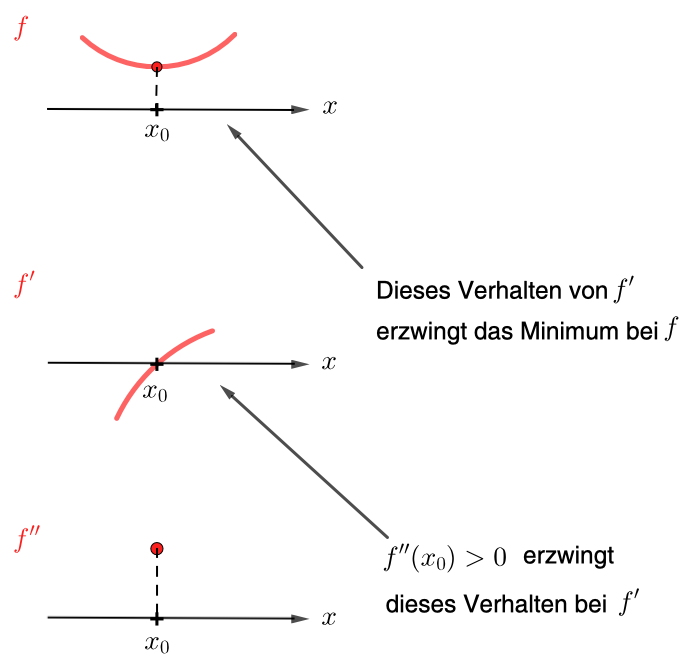
\includegraphics[width=\textwidth]{im/MinimumKriterium.png}
%     \end{center}
% \end{minipage}
% Analog können wir einsehen, dass $f'(x_0)=0$ zusammen mit $f''(x_0)<0$ ein (lokales) Maximum an der Stelle $x_0$ erzwingt.

% \begin{center}
%     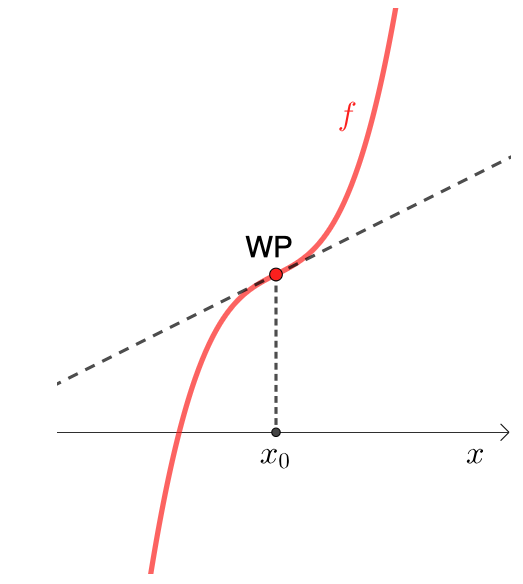
\includegraphics[width=0.4\textwidth]{im/WendepunktKruemmung.png}
% \end{center}

% \subsubsection*{Wendepunkte}
% Damit $f$ an einer Stelle $x_0$ einen Wendepunkt (erst rechts-, dann linksgekrümmt) aufweist, muss $f'$ an dieser Stelle ein (lokales) Minimum aufweisen. Warum? Wenn wir im Geiste die Tangente an obige Kurve legen und die Kurve von links nach rechts entlangfahren, so sehen wir, dass, wenn wir uns von links der Stelle $x_0$ nähern, die Steigungswerte sinken.

% Wir hatten ja vorher bemerkt, dass \glqq rechtsgekrümmt\glqq{} bedeutet, dass $f'$ im betrachteten Intervall streng monoton fallend ist. Die Steigungswerte sinken bis zu dem tiefsten Steigungswert, der zu der skizzierten Tangente an die Kurve im Wendepunkt gehört. Danach steigen sie wieder an. In dem nun folgenden linksgekrümmten Graphenabschnitt muss ja $f'$ streng monoton wachsen.

% Insgesamt sieht $f'$ lokal also so aus:
% \begin{center}
%     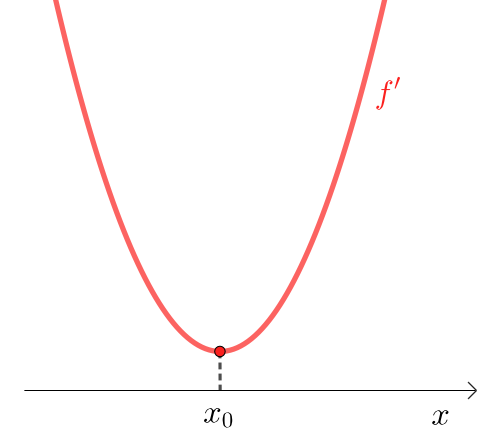
\includegraphics[width=0.3\textwidth]{im/WendepunktAbleitung.png}
% \end{center}
% $f'$ hat also an der Stelle $x_0$ ein lokales Minimum. Das bedeutet, dass die Ableitung von $f'$ (also $f''$) an der Stelle $x_0$ gleich $0$ sein muss, und die zweite Ableitung von $f'$ (also $f'''$) positiv sein muss. Somit ergibt sich: Ist $f''(x_0)=0$ und $f'''(x_0)>0$, dann hat $f$ an der Stelle $x_0$ einen Wendepunkt, in dem die Rechtskrümmung in eine Linkskrümmung übergeht.

% In analoger Weise gilt für einen Wendepunkt, wo die Linkskrümmung in eine Rechtskrümmung übergeht: $f''(x_0)=0$ und $f'''(x_0)<0$.
% \smallskip

% Zusammenfassend können wir für einen Wendepunkt folgendes Kriterium festhalten: $f''(x_0)=0,\ f'''(x_0)\neq 0$.

% Wenn nun zusätzlich noch $f'(x_0)=0$ gilt, so haben wir einen Terrassenpunkt, also einen Wendepunkt mit Steigung $0$.
% \begin{center}
%     \begin{tikzpicture}[scale=1.5]
%         % Achse
%         \draw[-{Latex}] (-1.6,0) -- (3.4,0) node[right] {$x$};

%         % Wendetangente
%         \draw[dashed, black]
%         plot[domain=-1.4:3.2] (\x, {1.3});

%         % Funktionsgraph (kubisch, WP bei x=1.2)
%         \draw[red, very thick, smooth, samples=100, domain=-0.7:2.7]
%         plot (\x, {0.22*(\x-1.2)^3 + 1.3});
%         \node[red] at (2.35,2.55) {$f$};

%         % Terrassenpunkt
%         \filldraw[red] (1.2,1.3) circle (2pt);
%         \node[above] at (1.2,1.55) {TP};

%         % Lot auf die x-Achse
%         \draw[dashed, gray!70!black] (1.2,1.3) -- (1.2,0);
%         \filldraw (1.2,0) circle (1.3pt);
%         \node[below] at (1.2,-0.1) {$x_0$};
%     \end{tikzpicture}
% \end{center}
\newpage
\subsubsection*{Zusammenfassung: Hinreichende Kriterien für spezielle Graphenpunkte}
\begin{table}[H]
    \centering
    \begin{tabular}{|c|c|c|}
        \hline
        \textbf{Hinreichende Bedingung}                                  & \textbf{Art des Punktes}                         & \textbf{Bild} \\
        \hline
        $f'(x_0) = 0; \ f''(x_0)< 0$                                     & Lokales Maximum / Hochpunkt an der Stelle $x_0$  &
        \raisebox{-0.5\totalheight}{\begin{tikzpicture}[line cap=round,line join=round,>=triangle 45,x=1cm,y=1cm]
                                            \begin{axis}[
                        x=0.2cm,y=0.2cm,
                        axis lines=middle,
                        xmin=-3.847508556384379,
                        xmax=11.34486704695043,
                        ymin=-6.469246379546205,
                        ymax=8.199581395348838,
                        xtick=\empty,
                        ytick=\empty,]
                    \clip(-3.847508556384379,-6.469246379546205) rectangle (11.34486704695043,8.199581395348838);
                    \draw [samples=50,rotate around={-180:(4.2,3.5)},xshift=0.84cm,yshift=0.7cm,line width=0.8pt,domain=-10:10)] plot (\x,{(\x)^2/2/2.5});
                    \begin{scriptsize}
                        \draw[color=black] (-1.5,-1.5) node {$f$};
                        \draw [line width=0.6pt] (4.2,-0.2)-- (4.2,0.2);
                        \draw[color=black] (4.355218955682325,-1.3) node {$x_0$};
                        \draw[color=black] (10.5,1) node {$x$};
                        \draw[color=black] (1,7) node {$y$};
                    \end{scriptsize}
                \end{axis}
                                        \end{tikzpicture}}                            \\
        \hline
        $f'(x_0) = 0; \ f''(x_0)> 0$                                     & Lokales Minimum / Tiefpunkt an der Stelle $x_0$  &
        \raisebox{-0.5\totalheight}{\begin{tikzpicture}[line cap=round,line join=round,>=triangle 45,x=1cm,y=1cm]
                                            \begin{axis}[
                        x=0.2cm,y=0.2cm,
                        axis lines=middle,
                        xmin=-3.847508556384379,
                        xmax=11.34486704695043,
                        ymin=-6.469246379546205,
                        ymax=8.199581395348838,
                        xtick=\empty,
                        ytick=\empty,]
                    \clip(-3.847508556384379,-6.469246379546205) rectangle (11.34486704695043,8.199581395348838);
                    \draw [samples=50,rotate around={-180:(4.2,3.5)},xshift=0.84cm,yshift=1cm,line width=0.8pt,domain=-10:10)] plot (\x,{-(\x)^2/2/2.5});
                    \begin{scriptsize}
                        \draw[color=black] (7,5) node {$f$};
                        \draw [line width=0.6pt] (4.2,-0.2)-- (4.2,0.2);
                        \draw[color=black] (4.355218955682325,-1.3) node {$x_0$};
                        \draw[color=black] (10.5,1) node {$x$};
                        \draw[color=black] (1,7) node {$y$};
                    \end{scriptsize}
                \end{axis}
                                        \end{tikzpicture}}                            \\
        \hline
        $f''(x_0) = 0; \ f'''(x_0)\neq 0$                                & Wendepunkt an der Stelle $x_0$                   &
        \raisebox{-0.5\totalheight}{\begin{tikzpicture}[line cap=round,line join=round,>=triangle 45,x=1cm,y=1cm]
                                            \begin{axis}[
                        x=0.2cm,y=0.2cm,
                        axis lines=middle,
                        xmin=-3.847508556384379,
                        xmax=11.34486704695043,
                        ymin=-6.469246379546205,
                        ymax=8.199581395348838,
                        xtick=\empty,
                        ytick=\empty,]
                    \clip(-3.847508556384379,-6.469246379546205) rectangle (11.34486704695043,8.199581395348838);
                    \draw[line width=1pt,color=black,smooth,samples=100,domain=-3.5:3,xshift=0.84cm,yshift=0.5cm] plot(\x,{0.2*(\x)^(3)+0.01*(\x)^(4)+0.2*(\x)});
                    \begin{scriptsize}
                        \draw[color=black] (7,5) node {$f$};
                        \draw [line width=0.6pt] (4.2,-0.2)-- (4.2,0.2);
                        \draw[color=black] (4.355218955682325,-1.3) node {$x_0$};
                        \draw[color=black] (10.5,1) node {$x$};
                        \draw[color=black] (1,7) node {$y$};
                    \end{scriptsize}
                \end{axis}
                                        \end{tikzpicture}}                            \\
        \hline
        \begin{minipage}{0.3\textwidth}
            \centering
            \[f'(x_0) = 0;\ f''(x_0) = 0\] \[f'''(x_0)\neq 0\]\end{minipage} & Sattelpunkt / Terrassenpunkt an der Stelle $x_0$ &
        \raisebox{-0.5\totalheight}{\begin{tikzpicture}[line cap=round,line join=round,>=triangle 45,x=1cm,y=1cm]
                                            \begin{axis}[
                        x=0.2cm,y=0.2cm,
                        axis lines=middle,
                        xmin=-3.847508556384379,
                        xmax=11.34486704695043,
                        ymin=-6.469246379546205,
                        ymax=8.199581395348838,
                        xtick=\empty,
                        ytick=\empty,]
                    \clip(-3.847508556384379,-6.469246379546205) rectangle (11.34486704695043,8.199581395348838);
                    \draw[line width=1pt,color=black,smooth,samples=100,domain=-3.5:3,xshift=0.84cm,yshift=0.5cm] plot(\x,{0.2*(\x)^(3)+0.01*(\x)^(4)});
                    \begin{scriptsize}
                        \draw[color=black] (7,5) node {$f$};
                        \draw [line width=0.6pt] (4.2,-0.2)-- (4.2,0.2);
                        \draw[color=black] (4.355218955682325,-1.3) node {$x_0$};
                        \draw[color=black] (10.5,1) node {$x$};
                        \draw[color=black] (1,7) node {$y$};
                    \end{scriptsize}
                \end{axis}
                                        \end{tikzpicture}}                            \\
        \hline
    \end{tabular}
\end{table}
\newpage
\subsubsection{Beispiele}
\begin{example}
    Hat die Funktion \[f(x)=\dfrac{8}{x}- \dfrac{16}{x^2}\] einen Hoch- oder Tiefpunkt?
    \kariert{40}
\end{example}
\newpage
Was bedeutet \textbf{hinreichend}? Am Beispiel des lokalen Maximum bedeutet es das Folgende: Wenn $f'\left(x_0\right)=0$ und $f''\left(x_0\right)<0$ dann hat die Funktion an der Stelle $x_0$ mit Sicherheit ein lokales Maximum. Umgekehrt aber nicht: Wenn die Funktion an der Stelle $x_0$ ein lokales Maximum hat, dann folgt nicht unbedingt, dass die zweite Ableitung negativ ist: $f''(x_0)$ könnte auch $0$ sein. Das ist bei der Funktion $f\left(x\right)=-x^4$ zum Beispiel der Fall.
\begin{example}
    Untersuche die Funktion \[f(x)=x^4-1\]
    \kariert{40}
\end{example}
\newpage
\subsection{Aufgaben}
% \begin{enumerate}

%     \item Wir wissen von der Ableitung $f'$ einer Funktion $f$, dass sie auf dem ganzen Intervall
%           $[2,3]$ existiert und negativ ist. Wo in diesem Intervall hat dann die Funktion $f$ ihren
%           maximalen Funktionswert? Und warum?

%           \begin{itemize}
%               \item An der Stelle $x=2$.
%               \item An der Stelle $x=3$.
%               \item An einer Stelle $x$ mit der Eigenschaft $2<x<3$.
%               \item Die Funktion $f$ hat auf diesem Intervall keinen maximalen Funktionswert,
%                     weil die Ableitung nie $0$ ist.
%               \item Wir wissen nicht, ob $f$ auf diesem Intervall ein Maximum hat, da nicht bekannt ist, wo die zweite Ableitung negativ ist.
%           \end{itemize}

%     \item Sei
%           \[
%               f(x)=x^5-x.
%           \]
%           Weisen Sie nach, dass

%           \begin{enumerate}
%               \item der Graph rechtsgekrümmt im Intervall $]-\infty,0]$ und linksgekrümmt im Intervall
%                     $[0,\infty[$ ist.

%               \item die Funktion genau einen Wendepunkt an der Stelle $x=0$ hat.
%                     Mit welcher $y$-Koordinate?

%               \item die Funktion ein lokales Maximum an der Stelle
%                     \[
%                         x=-\sqrt[4]{0.2}
%                     \]
%                     und ein lokales Minimum an der Stelle
%                     \[
%                         x=\sqrt[4]{0.2}
%                     \]
%                     hat.
%           \end{enumerate}

%     \item Sei
%           \[
%               g(x)=\frac{1}{12}x^4-\frac{5}{6}x^3+2x^2.
%           \]
%           Können Sie nachweisen, dass diese Funktion genau zwei Wendepunkte hat?
%           An welchen Stellen und mit welchen $y$-Koordinaten?
%           Um was für Typen von Wendepunkten handelt es sich?

%     \item Sei
%           \[
%               h(x)=-\frac{1}{6}x^3+2x+3.
%           \]
%           Bitte weisen Sie nach, dass

%           \begin{enumerate}
%               \item $(0,3)$ der einzige Wendepunkt dieser Funktion ist und dass der Graph links davon
%                     linksgekrümmt und rechts davon rechtsgekrümmt ist.

%               \item es ein lokales Minimum an der Stelle $x=-2$ und ein lokales Maximum an der Stelle
%                     $x=2$ gibt. Mit welchen $y$-Koordinaten?
%           \end{enumerate}

%     \item Sei
%           \[
%               k(x)=x^3-6x^2+12x-7.
%           \]
%           Können Sie nachweisen, dass diese Funktion einen Terrassenpunkt an der Stelle
%           $x=2$ hat?

% \end{enumerate}
\begin{enumerate}
    \item Bestimme die Extrema (= Hoch- und Tiefpunkte) der Funktion  $$ f(x) = x^3 + 6x^2 - 15x + 19$$
    \item  Gegeben ist die Funktion \( f \) mit \( f(x) = x^3 + 3x^2 - 4 \).
          \begin{enumerate}
              \item Bestimme vom Graphen der Funktion \( f \) alle Tief-, Hoch- und Wendepunkte.
              \item Gib jeweils die Intervalle an, in welchen der Graph der Funktion \( f \) monoton steigt bzw. fällt.
              \item Skizziere den Graphen \( G_f \).
          \end{enumerate}
    \item Von der Funktion \( f \) ist die Funktionsgleichung
          \[
              f(x) = 3x^4 - 8x^3 + 6x^2
          \]
          gegeben.
          \begin{enumerate}
              \item Berechne in den Wendepunkten der Funktion \( f \) die Geradengleichungen der Tangenten (sogenannte `Wendetangenten').
              \item In welchem Intervall ist der Graph von \( f \) links- bzw. rechtsgekrümmt?
          \end{enumerate}
    \item Zu hinreichende und notwendige Bedingungen: Bestimme die Extrema und Wendepunkte der Kurve $y=x^6-12x^5$.

    \item Welche Art Punkt hat die Kurve
          $$ y= \frac{1}{5} x^5 - x^4 + 2x^3 -2 x^2 + x - 1$$
          an der Stelle $x=1$?
    \item Bestimme $k\in \R$, sodass $y=x^3+kx^2+2$ bei $x= 3$ einen Wendepunkt hat.
    \item Für welchen Wert von $a\in\R$ hat die Funktion $f(x) = x^2 + \frac{a}{x}$ an der Stelle $x=-1$ ein Extremum? \\
          Handelt es sich um einen Tief- oder um einen Hochpunkt
\end{enumerate}
\newpage
\subsubsection*{Lösungen}
\begin{enumerate}
    \item $H=(-5, 119), T=(1,11)$
    \item \begin{enumerate}
              \item $H=(-2, 0), T=(0, -4), W=(-1, -2)$
              \item Fallend: $]-2, 0[$, steigend $\R \setminus ]-2, 0[$
              \item \dots
          \end{enumerate}
    \item \begin{enumerate}
              \item $t_1: y= \frac{16}{9}x -\frac{5}{27}, \quad t_2: y=1$
              \item Rechtsgekrümmt: $]\frac{1}{3}, 1[$ linksgekrümmt $\R \setminus ]\frac{1}{3}, 1[$
          \end{enumerate}

    \item $T=(10, -200000), S =(0,0), W=(8, -131072)$
    \item Einen Sattelpunkt.
    \item $k= -9$
    \item $a=-2$, Tiefpunkt.

\end{enumerate}
\clearpage

\subsection{Kurvendiskussion}
Das Ziel einer sogenannten `Kurvendiskussion' ist es, den Graphen einer Funktion möglichst genau zu beschreiben. Dazu werden in der Regel die folgenden Eigenschaften des Graphen/der Funktion bestimmt:
\begin{enumerate}
    \item Definitionsbereich und allfällige Symmetrie zum Ursprung oder zur $y$-Achse.
    \item Achsenschnittpunkte.
    \item Ableitungen.
    \item Extrema, Wende- und Sattelpunkte.
    \item Asymptotisches Verhalten für $x\to\pm\infty$ und an den Definitionslücken.
    \item Skizze des Graphs.
\end{enumerate}

\begin{example}
    Diskussion der Funktion $f(x) = \frac{8x-16}{x^2}$
\end{example}
\kariert{34}

\pagebreak

\kariert{52}

\pagebreak

\kariert{52}

\clearpage
\subsubsection{Übungen}
\begin{enumerate}
    \item
          Führen Sie eine Kurvendiskussion für die folgenden Polynomfunktionen durch
          \begin{enumerate}
              \item $f(x) = \frac{1}{3}\left(4x^3-x^4\right)$
              \item $g(x) = \frac{1}{3}\left(x^4-8x^3+18x^2\right)$
              \item $h(x) = \frac{1}{25}\left(x^4-32x^2+31\right)$
          \end{enumerate}
    \item Anspruchsvolle Aufgabe: Führen Sie eine Kurvendiskussion für die folgenden nicht-polynomialen Funktionen durch
          \begin{enumerate}
              \item $a(x) = \left(\frac{x-1}{x+1}\right)^2$
              \item $b(x) = \frac{1}{x} - \frac{1}{\sqrt x}$
              \item $c(x) = \sin(x) + 2\cos(x) $
              \item $d(x) = e^x (x-1)^2$
              \item $f(x) = x\ln(x)$
          \end{enumerate}
\end{enumerate}

\clearpage
\subsubsection*{Lösungen}

\begin{enumerate}
    \item
          Führen Sie eine Kurvendiskussion für die folgenden Polynomfunktionen durch
          \begin{enumerate}
              \item $f(x) = \frac{1}{3}(4x^3 - x^4)$
                    \begin{itemize}
                        \item $D_f = \mathbb{R}$, keine Symmetrie
                        \item $Y = (0, 0)$, Nullstellen: $N_1 = (0, 0)$, $N_2 = (4, 0)$
                        \item $f'(x) =\frac{1}{3}(12x^2 - 4x^3) , f''(x)=\frac{1}{3}(24x - 12x^2)$ \dots
                        \item Extrema: $H = (3, 9)$ \\
                              Wendepunkte: $W = (2, \frac{16}{3})$
                              Sattelpunkt $S = (0, 0)$
                        \item $\lim\limits_{x \to \pm\infty} f(x) = -\infty$
                    \end{itemize}

              \item $g(x) = \frac{1}{3}(x^4 - 8x^3 + 18x^2)$
                    \begin{itemize}
                        \item $D_g = \mathbb{R}$, keine Symmetrie
                        \item $Y = (0, 0)$, Nullstellen: $N = (0,0)$
                        \item $g'(x)= \frac{1}{3}(4x^3 - 24x^2 + 36x), g''(x)= \frac{1}{3}(12x^2 - 48x + 36)$ \dots
                        \item Extrema: $T=(0, 0)$ \\
                              Wendepunkte: $W_1 = (1, \frac{11}{3})$
                              Sattelpunkt $S = (3, 9)$
                        \item $\lim\limits_{x \to \pm\infty} g(x) = \infty$
                    \end{itemize}

              \item $h(x) = \frac{1}{25}(x^4 - 32x^2 + 31)$
                    \begin{itemize}
                        \item $D_h = \mathbb{R}$ , $f(-x) = f(x)$ symmetrisch zur $y$-Achse.
                        \item $Y = (0, 1.24)$, Nullstellen: $N = \{-5.57, -1, 1, 5.57\}$
                        \item $h'(x) = \frac{1}{25}(4x^3 - 64x), h''(x)= \frac{1}{25}(12x^2 - 64)$
                        \item Extrema: $T_1 = (-4, -9)$, $H_1 = (0, 1.24)$, $T_2 = (4, -9)$ \\
                              Wendepunkte: $W_1 = (-2.31, -4.45)$, $W_2 = (2.31, -4.45)$
                        \item $\lim\limits_{x \to \pm\infty} h(x) = \infty$
                    \end{itemize}
          \end{enumerate}


    \item 
          \begin{enumerate}
              \item \( a(x) = \left( \frac{x - 1}{x + 1} \right)^2 \):
                    \begin{itemize}
                        \item $D_a = \mathbb{R} \setminus \{1\}$ , keine Symmetrie
                        \item $Y = (0, 1)$, Nullstellen: $N = (1,0)$
                        \item $a'(x) = 4 \frac{x-1}{(x+1)^3}, a''(x) =  8 \frac{2-x}{(x+1)^4}$
                        \item Extrema: $T=(1, 0)$ \\
                              Wendepunkte: $W = (2, \frac{1}{9})$
                        \item $\lim\limits_{x \to \pm\infty} a(x) = 1$ \\
                              $\lim\limits_{x \nearrow -1} a(x) = \lim\limits_{x \searrow -1} a(x)=\infty $
                    \end{itemize}
              \item \( b(x) = \frac{1}{x} - \frac{1}{\sqrt{x}} \):
                    \begin{itemize}
                        \item $D_b = \mathbb{R}^+ $ , keine Symmetrie
                        \item Nullstelle: $N = (1,0)$
                        \item $b'(x) = \frac{\sqrt{x}-2}{2x^2}, b''(x) =  \frac{-3\sqrt{x}+8}{4x^3}$
                        \item Extrema: $T=(4, -\frac{1}{4})$ \\
                              Wendepunkte: $W = (\frac{64}{9}, -\frac{15}{64})$
                        \item $\lim\limits_{x \to \infty} b(x) = 0$ \\
                              $\lim\limits_{x \searrow 0} b(x)=\infty $
                    \end{itemize}
              \item \( c(x) = \sin(x) + 2\cos(x) \):
                    \begin{itemize}
                        \item $D_c = \mathbb{R}$ , keine (einfache( Symmetrie
                        \item $Y = (0, 2)$, Nullstellen: $N = (2.03 +k\cdot \pi,0), k\in \mathbb{Z}$
                        \item $c'(x) = \cos(x) - 2 \sin(x), c''(x) =  -\sin(x)-2\cos(x)$
                        \item Extrema: $T=(3.61+2k\pi, -2.24), H=(0.46+2k\pi, 2.24)$ \\
                              Wendepunkte: $W = (2.03 + k\pi, 0)$
                        \item $\lim\limits_{x \to \pm\infty} c(x) $ existiert nicht.
                    \end{itemize}
              \item \( d(x) = e^x(x - 1)^2 \):
                    \begin{itemize}
                        \item $D_d = \mathbb{R}$ , keine Symmetrie
                        \item $Y = (0, 1)$, Nullstellen: $N = (1,0)$
                        \item $d'(x) = e^x(x^2-1), d''(x) = e^x (x^2+2x-1)$
                        \item Extrema: $T=(1,0), H=(-1, \frac{4}{e})$ \\
                              Wendepunkte: $W_1 = (-\sqrt{2}-1, 1.04), W_2 =(\sqrt{2}-1, 0.52)$
                        \item $\lim\limits_{x \to \infty} d(x) = \infty, \lim\limits_{x \to -\infty} d(x) = 0$
                    \end{itemize}
              \item \( f(x) = x\ln(x) \):
                    \begin{itemize}
                        \item $D_f = \mathbb{R^+}$, keine Symmetrie
                        \item Nullstellen: $N = (1,0)$
                        \item $f'(x) = \ln(x) + 1, f''(x) = \frac{1}{x}$
                        \item Extrema: $T=\left(\frac{1}{e}, -\frac{1}{e}\right)$
                        \item $\lim\limits_{x \to \infty} f(x) = \infty$ \\
                              $\lim\limits_{x \searrow 0} f(x) = 0$ (Für die Berechnung dieses Grenzwertes benötigt man spezielle Techniken
                    \end{itemize}
          \end{enumerate}
\end{enumerate}

\clearpage
\subsection{Weitere Übungen}
\begin{enumerate}
    \item In welchen Punkten verläuft die Kurventangente des Graphen von $f(x) = \frac{1}{3} x^3-x^2+x-4$ senkrecht zur Geraden $p: y=-\frac{1}{4}x+42$?
    \item Bestimme die Extrema und Wendepunkte der Funktion:
          \begin{enumerate}
              \item $f(x) = x^4-4x^3+4x^2$
              \item $g(x) = x + \frac{1}{x+1}$
          \end{enumerate}
    \item Eine Gleichung $n$-ten Grades hat höchstens $n$ Lösungen (\emph{Fundamentalsatz der Algebra}). \\
          Wie viele Extrema hat eine Polynomfunktion $n$-ten Grades höchstens? Und wie viele Wendepunkte?
    \item Führe eine Kurvendiskussion durch für
          \begin{enumerate}
              \item $f(x) = x^3-3x$
              \item $g(x) = x^3\cdot e^{-x}$
          \end{enumerate}
\end{enumerate}

\clearpage
\subsubsection*{Lösungen}
\begin{enumerate}
    \item \begin{enumerate}
              \item $t: y=8x-13 \quad n: y= -\frac{1}{8}x +\frac{26}{8}$
              \item $t: y=\frac{1}{2}x-\frac{7}{2} \quad n: y= -2x -11$
              \item $t: y=\frac{1}{4}x+1 \quad n: y= -4x +18$
          \end{enumerate}
    \item \begin{enumerate}
              \item $\varphi\approx 26.6^\circ$
              \item $\varphi_1=\varphi_2\approx 18.9^\circ$
              \item $\varphi\approx 63.4^\circ$
          \end{enumerate}
    \item $P_1 =\left(-1, -\frac{19}{3}\right), P_2 = (3,-1 )$
    \item \begin{enumerate}
              \item $T_1 = (0,0), W_1 \approx(0.42, 0.44) , H =(1,1), W_2\approx(1.58, 0.44), T_2=(2,0)$
              \item $T=(0, 1), H = (-2, -3)$, keine Wendepunkte.
          \end{enumerate}
    \item Höchstens $n-1$ Extrema und $n-2$ Wendepunkte.
    \item \begin{enumerate}
              \item \begin{itemize}
                        \item $D = \mathbb{R}$ , Punktsymmetrisch zum Ursprung ($f(-x) = -f(x)$)
                        \item $Y = (0, 0)$, Nullstellen: $N_1 = (0,0), N_{2,3} = (\pm \sqrt{3}, 0)$
                        \item $f'(x) =3x^2-3, f''(x) = 6x$
                        \item Extrema: $T=(1,-2), H=(-1, 2)$ \\
                              Wendepunkte: $W = (0, 0)$
                        \item $\lim\limits_{x \to \infty} f(x) = \infty, \lim\limits_{x \to -\infty} f(x) = -\infty$
                    \end{itemize}
              \item \begin{itemize}
                        \item  $D = \mathbb{R}$
                        \item $Y = (0, 0)$, Nullstellen: $N = (0,0)$
                        \item $g'(x) = e^{-x} (3x^2-x^3), g''(x) = e^{-x} (x^3-6x^2+6x)$
                        \item Extrema: $ H=(3, 1.34)$ \\
                              Wendepunkte: $W_1 \approx (1.27, 0.57), W_2 \approx(4.73, 0.93)$ \\
                              Sattelpunkt $S=(0,0)$
                        \item $\lim\limits_{x \to \infty} g(x) =0, \lim\limits_{x \to -\infty} g(x) = -\infty$
                    \end{itemize}
          \end{enumerate}


\end{enumerate}